\section{Research Methodology} \label{method}

In this chapter the methodology used to develop random forest model will be discussed. The details of fusion between AIS data, ECMWF and CMEMS data source used for training the model will be presented in \Cref{data_acquisition}. Suitable methodology application during data pre-processing will be described in \Cref{data_prep_sub}. The selection for appropriate, domain knowledge based, feature selection will be explained in \Cref{feature_select}. The selection of the most optimal model hyperparameter for different tree-based model will be explained in \Cref{hpo}. To validate the model's generalisation capability, statistical performance measure is used. The underlying principle is elaborated in \Cref{model_validation}. Summary of methodology application in this study is summarised in \Cref{methodology_application} and visually represented in figure \Cref{fig:flowchart}. 

\begin{figure}[h]
    \centering
        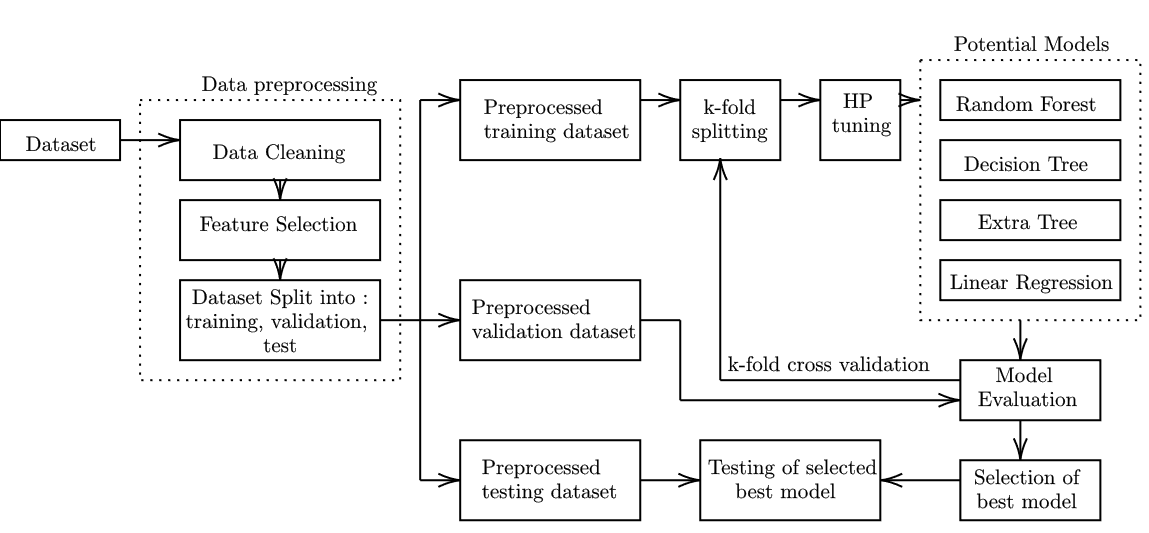
\includegraphics[width=\textwidth]{02_figures/flowmethod2.png}
        \caption{Scheme of proposed methodology}
        \label{fig:flowchart}
\end{figure}

\subsection{Data Acquisition}\label{data_acquisition}

For the purpose of model training, 2021 AIS data from Ro-Ro ferry ship Hammershus is collected. The shore-based AIS data is made available by Danish Maritime Authority which tracked her journey between ports of K{\o}ge, R{\o}nne, Ystad and Sassnitz and structured according to \Cref{AIS_struct}. The AIS data is fused with weather data from ECMWF\footnote{European Centre for Medium-Range Weather Forecast} with temporal resolution of 1 hour at granularity of 0.25° (longitude) x 0.25° (latitude), data from ECMWF provides information for wind, waves and seawater temperature. The information for current is obtained from CMEMS\footnote{Copernicus Marine Environment Monitoring Service} with temporal resolution of 3 hours at granularity of  0.25° (longitude) x 0.25° (latitude).\\ 

The resulting fusion resulted in dataset with temporal resolution of 1 hour. Some information static information from the AIS data are excluded before further data preprocessing, this includes ship's MMSI, Callsign, Name, IMO and Navigational Status. Additionally, information of the ship's Rate of Turn (ROT) is not available in this case. The weather information is synchronised so that the wind, waves, seawater temperature and sea current belongs to the same weather grid with same temporal resolutions.\\ 

Through vector decomposition, information of Northward and Eastward wind velocity is converted to absolute wind speed and wind direction \emph{with respect to True North},$\varphi$. Similarly, information of Northward and Eastward current Velocity is converted to absolute current speed and current direction \emph{with respect to True North} $\gamma$.\\ 

Additional information is then added to the dataset. True direction information is added to gain information of the effect of weather direction \emph{with respect to ship's beam}. As such, from information based on True North such as: wind direction, current direction, swell direction, wind wave direction and true wave direction, are converted to information on true direction and added to the dataset. The initial structure have 32 features, 9 AIS feature and 23 weather features. The structure of the initial dataset i.e. before data preprocessing and feature selection, is summarised in \Cref{dataset_init_struct} \\

\begin{table}
    % \small
    % \centering
    % \resizebox {\textwidth}{!}
    {\begin{tabular}{ |p{8cm}|c| }
    \hline
    \textbf{Feature} & \textbf{Unit} \\
    \hline
    \multicolumn{2}{|l|}{\textbf{AIS data}}\\
    \hline
    Position Time Stamp & DD\slash MM\slash YYYY HH:MM:SS\\
    \hline
    Latitude & $deg.$\\
    \hline
    Longitude & $deg.$ \\
    \hline
    Width & $m$ \\
    \hline
    Length & $m$ \\
    \hline
    SOG & $\text{knot}$ \\
    \hline
    COG & $deg.$ \\
    \hline
    Heading & $deg.$ \\
    \hline
    Draught & $m$ \\
    \hline
    \multicolumn{2}{|l|}{\textbf{Weather Data (0.5° Granularity)}}\\
    \hline
    Wind Speed & $m/s$ \\
    \hline
    True North Wind Direction $\varphi$ & $m/s$ \\
    \hline
    Temperature above oceans & $K$ \\
    \hline
    Air Density above oceans & $kg/m^3$\\
    \hline
    Maximum Wave Height & $m$ \\
    \hline
    Swell Direction & $deg.$\\
    \hline
    Wind Wave Direction & $deg.$ \\
    \hline
    Swell Period & $deg.$ \\
    \hline
    Wind Wave Period & $sec$\\
    \hline
    Wave Direction & $deg.$\\
    \hline
    Wave Period & $sec.$\\
    \hline
    Sea Surface Temperature & $K$\\
    \hline
    Combined Wind Wave Swell Height & $m$ \\
    \hline
    Swell Height & $m$\\
    \hline
    Wind Wave Height & $m$ \\
    \hline
    Surface Pressure & $Pa$ \\
    \hline
    Current Speed & $m/s$\\
    \hline
    True North Current Direction $\gamma$ & $m/s$\\
    \hline
    True Wind Direction & $deg.$ \\
    \hline
    True Current Direction & $deg.$ \\
    \hline
    True Swell Direction & $deg.$ \\
    \hline
    True Wind Wave Direction & $deg.$ \\
    \hline
    True Wave Direction & $deg.$ \\
    \hline
    \end{tabular}}
\caption{Structure of fused dataset}\label{dataset_init_struct}
\end{table}

\subsubsection{Data Preprocessing}\label{data_prep_sub}




\subsection{Feature Selection}\label{feature_select}

\subsection{Modelling}\label{modelling}

\subsubsection{Model Hyperparameter Optimisation}\label{hpo}

\subsubsection{Model Validation}\label{model_validation}

\subsubsection{Methodology Application}\label{methodology_application}



\begin{itemize}
    \item Two data sources are imported. {\tt AIS\_weather\_H\_ok2\_copy.csv} \\ and {\tt AIS\_weather\_h\_rename\_copy.csv}. The information from the latter comma delimited 
    file will be used for calculating the ship Speed Through Water (STW).  
    The information required is the true north current direction. Which is obtained from the vector component of the Northward and Southward current.
    \item This dataframe will be merged with the main dataframe from \\ the file {\tt AIS\_weather\_H\_ok2\_copy.csv}.
    \item Omission of the journey data between Ronne and Sassnitz
    \item SOG threshold is applied to omit ship mooring and maneuvering to accurately represent the ship's steady state operation 
    \cite{Abebe.2020,BalBesikci.2016,Gkerekos.2019,Yang.2020}. This threshold is selected as 5 knots according to \cite{Abebe.2020}
    \item The AIS data from June is filtered. This data will be used as validation data to check the model's performance.
\end{itemize}
 
\subsection{Data Analysis}
\begin{itemize}
    \item The features are represented in a histogram plot. For the feature Current speed, anomaly is detected. Certain spike is detected around $0.01 - 0.03$ \verb|m/s|. Reasons unknown. The data is retained, including the spike, until a definitive answer can be found.
    \item OPEN QUESTION : What is the necessity of feature standardization / normalization ? Normalization is required for ANN as model training requires the value between 0 and 1. But in case of RFR, there is no such requirement. Through testing, data standardization also does not seem to improve the model's performance. 
\end{itemize}

\begin{sidewaysfigure}
    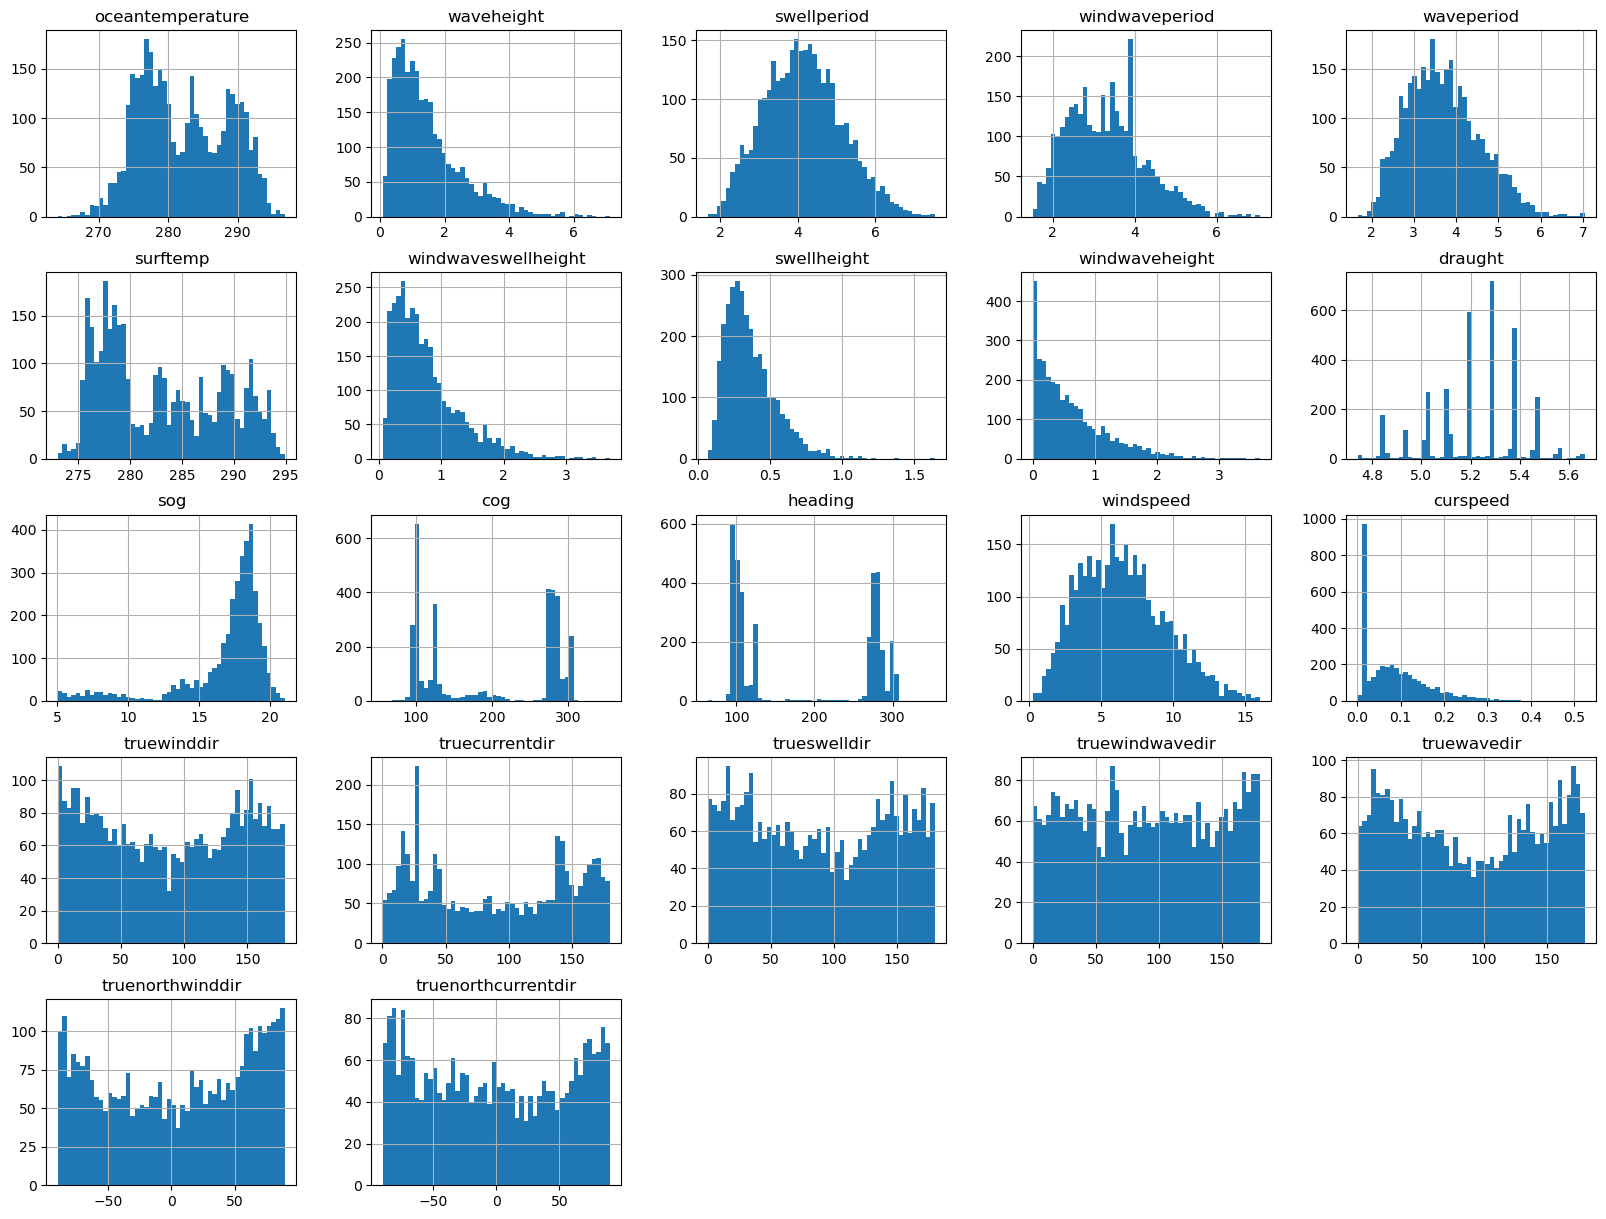
\includegraphics[width=\linewidth,height=\textheight,keepaspectratio]{02_figures/outputhist.png}
    \caption{Histogram of the features}
    \label{sidewaysfig:hist1}
\end{sidewaysfigure}

\newpage

\begin{itemize}
    \item The correlation of the features against SOG are determined. It is found that :
    \begin{itemize}
        \item Draught
        \item Course Over Ground (COG)
        \item heading
        \item Wind Speed
        \item Current Speed
        \item True Current direction
    \end{itemize}
    Have relatively stronger correlation to SOG compared to other features, albeit the correlation is a weak one
    \item The correlation between the features is displayed using the following the heat map. From the heat map it can be observed that between these features:
    \begin{itemize}
        \item Waveheight and wind wave swell height
        \item Waveheight and wind wave height
        \item Windwaveswellheight and wave period
    \end{itemize}
    Have a strong correlation between each other.  
    \item Open topic: 
    \begin{itemize}
        \item Feature reduction is possible, \cite{Abebe.2020} suggested high feature correlation filter, the filter suggest that two features which has a high correlation $(>90\%)$ is to be combined into a single feature. But the author is unsure whether this combination is physically sensible. Hence, this filter is yet to be applied for feature reduction. 
        \item Some of these features can be connected through wave equations, but the author has not found an equation which could relate these features.
    \end{itemize}
    \item The random forest regressor could not function when \verb|NaN| values are present. With that, the missing values are filled in using the {\tt imputer} function. The missing values are filled in by means of \verb|KNN|.
\end{itemize}

\newpage

\begin{figure}[h]
    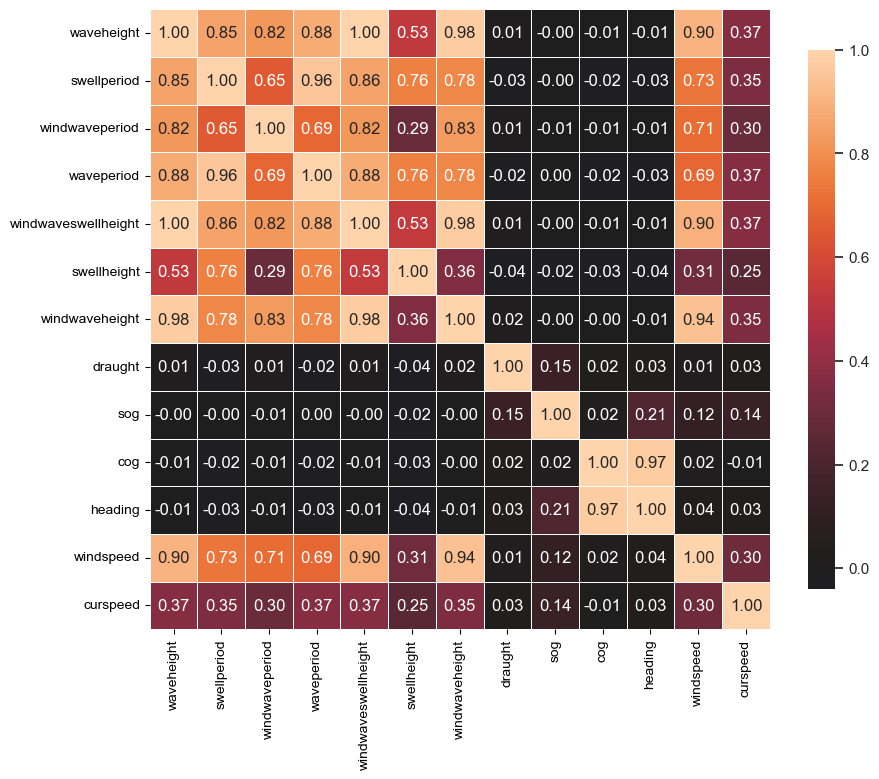
\includegraphics[width=\linewidth,height=\textheight,keepaspectratio]{02_figures/heatmap_corr.png}
    \caption{Correlation Heat Map}
    \label{fig:heatmap1}
\end{figure}

\subsection{Modelling}

\begin{itemize}
    \item The data is split into 80:20 ratio. But considering the validation data, it is split into approximately 73:18:9.
    \item The model is then trained using Random Forest Regression (RFR). Additional training is also performed using Decision Tree Regressor (DTR). DTR model performance will be used as a benchmark as it is also a tree-based modelling method with similar methodology to RFR.
    \item The computational time of DTR is significantly faster than RFR
    Model Evaluation    
\end{itemize}

\subsection{Predicting STW}
\begin{itemize}
    \item The ship's Speed Through Water STW can be calculated using vector component of the SOG and current speed. The direction used will be according to True North. \cite{Yang.2020,Zhou.2020}
    \item SOG represents the speed of the ship with reference to the ground, while the STW represent the ship's speed with reference to water.
    \item SOG also can be termed by the ship's speed that is captured by the GPS, and does not consider any effect of the current
    \item This means that the ship's STW will be greater than the ship's SOG when there is current moving against the ship's movement direction and vice versa 
    \item The vector decomposition can be defined from the following equations, which is based on the equation by \cite{Yang.2020}:
    \begin{itemize}
        \item The ship's SOG $V_g$ can be decomposed into $V_{g}^x$ and $V_{g}^y$, which represents the $x$ and $y$ components of the SOG respectively using the ship's course heading (COG) $\beta$ \emph{with respect to True North}:
        \begin{equation}\label{eqvgx}
            V_{g}^x = V_g\sin(\beta)   
        \end{equation}
        \begin{equation}\label{eqvgy}
            V_{g}^y = V_g\cos(\beta)   
        \end{equation}
        \item To consider the effect of sea current. The current speed $V_c$ will also be decomposed to $x$ and $y$ components respectively using the current direction $\gamma$ \emph{with respect to True North}:
        \begin{equation}\label{eqvcx}
            V_{c}^x = V_g\sin(\gamma)   
        \end{equation}
        \begin{equation}\label{eqvcy}
            V_{c}^y = V_g\cos(\gamma)   
        \end{equation}
        \item from here the ship' STW $V_{wx}$ and $V_{wy}$ component can be found from the following equation: 
        \begin{equation}
            V_{w}^x = V_{g}^x - V_{c}^x    
        \end{equation}
        \begin{equation}
            V_{w}^y = V_{g}^y - V_{c}^y 
        \end{equation}
        \item The magnitude of the STW can be readily obtained from the following vector synthesis
        \begin{equation}
            V_w = \sqrt{(V_{w}^x)^2 + (V_{w}^y)^2} 
        \end{equation}
    \end{itemize}
    \newpage

    \item This principle is applied to the following Python script. \ref{eqvcx}

\begin{python}
       
        # Convert SOG from [Knots] to [m/s]
    
        dfprog["vgms"] = dfprog["sog_pred"]/1.9438
        
        # Convert the angles from [Degrees] to [Radians]

        rad_gamma = np.deg2rad(dfprog["gamma"])
        rad_cog = np.deg2rad(dfprog["cog"])

        # Decomposition in x-component

        dfprog["vgx"] = dfprog["vgms"] * np.sin(rad_cog)
        dfprog["vcx"] = dfprog["curspeed"] * np.sin(rad_gamma)
        dfprog["stw_x"] = (dfprog["vgx"] - dfprog["vcx"])

        # Decomposition in y-component

        dfprog["vgy"] = dfprog["vgms"] * np.cos(rad_cog)
        dfprog["vcy"] = dfprog["curspeed"] * np.cos(rad_gamma)
        dfprog["stw_y"] = (dfprog["vgy"] - dfprog["vcy"])

        # Vector synthesis and reconversion to [Knots] from [m/s]

        dfprog["vwms_p"] = np.sqrt(dfprog["stw_x"]**2 + dfprog["stw_y"]**2)
        dfprog["stw_pred"] = dfprog["vwms_p"]*1.9438  

    \end{python}
\newpage

\begin{sidewaysfigure}
    \includegraphics[width=\linewidth,height=\textheight,keepaspectratio]{02_figures/rfrftree.png}
    \caption{Correlation Heat Map}
    \label{fig:Random Forest Regression Tree}
\end{sidewaysfigure}


\end{itemize}
